\documentclass{article}\usepackage[]{graphicx}\usepackage[]{xcolor}
% maxwidth is the original width if it is less than linewidth
% otherwise use linewidth (to make sure the graphics do not exceed the margin)
\makeatletter
\def\maxwidth{ %
  \ifdim\Gin@nat@width>\linewidth
    \linewidth
  \else
    \Gin@nat@width
  \fi
}
\makeatother

\definecolor{fgcolor}{rgb}{0.345, 0.345, 0.345}
\newcommand{\hlnum}[1]{\textcolor[rgb]{0.686,0.059,0.569}{#1}}%
\newcommand{\hlsng}[1]{\textcolor[rgb]{0.192,0.494,0.8}{#1}}%
\newcommand{\hlcom}[1]{\textcolor[rgb]{0.678,0.584,0.686}{\textit{#1}}}%
\newcommand{\hlopt}[1]{\textcolor[rgb]{0,0,0}{#1}}%
\newcommand{\hldef}[1]{\textcolor[rgb]{0.345,0.345,0.345}{#1}}%
\newcommand{\hlkwa}[1]{\textcolor[rgb]{0.161,0.373,0.58}{\textbf{#1}}}%
\newcommand{\hlkwb}[1]{\textcolor[rgb]{0.69,0.353,0.396}{#1}}%
\newcommand{\hlkwc}[1]{\textcolor[rgb]{0.333,0.667,0.333}{#1}}%
\newcommand{\hlkwd}[1]{\textcolor[rgb]{0.737,0.353,0.396}{\textbf{#1}}}%
\let\hlipl\hlkwb

\usepackage{framed}
\makeatletter
\newenvironment{kframe}{%
 \def\at@end@of@kframe{}%
 \ifinner\ifhmode%
  \def\at@end@of@kframe{\end{minipage}}%
  \begin{minipage}{\columnwidth}%
 \fi\fi%
 \def\FrameCommand##1{\hskip\@totalleftmargin \hskip-\fboxsep
 \colorbox{shadecolor}{##1}\hskip-\fboxsep
     % There is no \\@totalrightmargin, so:
     \hskip-\linewidth \hskip-\@totalleftmargin \hskip\columnwidth}%
 \MakeFramed {\advance\hsize-\width
   \@totalleftmargin\z@ \linewidth\hsize
   \@setminipage}}%
 {\par\unskip\endMakeFramed%
 \at@end@of@kframe}
\makeatother

\definecolor{shadecolor}{rgb}{.97, .97, .97}
\definecolor{messagecolor}{rgb}{0, 0, 0}
\definecolor{warningcolor}{rgb}{1, 0, 1}
\definecolor{errorcolor}{rgb}{1, 0, 0}
\newenvironment{knitrout}{}{} % an empty environment to be redefined in TeX

\usepackage{alltt}
\usepackage{hyperref}
\usepackage[margin=1in]{geometry}
\usepackage{booktabs}
\usepackage{amsmath}
\usepackage{gensymb}
\usepackage{natbib}
\usepackage{parskip}
\usepackage{longtable}
\usepackage{lineno}
\usepackage{makecell}
\usepackage{setspace}

\setcounter{secnumdepth}{0} 

\setlength{\parindent}{0pt}
\IfFileExists{upquote.sty}{\usepackage{upquote}}{}
\begin{document}
% \SweaveOpts{concordance=TRUE}
\linenumbers
\setstretch{2}

\begin{center}
{\sc} {\Large Supplementary Material} \\
\vspace{5ex}
{\sc} Christophe Rouleau-Desrochers$^1$*, Victor Van der Meersch$^1$, D.M. Buonaiuto$^{2,3,5}$, C.J. Chamberlain$^{2,3,4}$, Deirdre Loughnan$^1$, Neil Pederson$^6$, \& E.M. Wolkovich$^{1,2,3}$
\end{center}
$^1$Forest \& Conservation Sciences, Faculty of Forestry \& Environmental Stewardship, University of British Columbia, Vancouver, British Columbia, Canada\\
$^2$Arnold Arboretum of Harvard University, Boston, Massachusetts, USA\\
$^3$Department of Organismic and Evolutionary Biology, Harvard University, Cambridge, Massachusetts, USA\\
$^4$The Nature Conservancy, Durham, North Carolina, USA\\
$^5$Department of Plant Science and Landscape Architecture, University of Maryland, College Park, Maryland, USA \\
$^6$Highstead Foundation, Redding, Connecticut, USA \\
*crouleau@alum.ubc.ca

% Set Wildchrokie species shortcut
\newcommand{\Ainc}{\textit{A. incana}}
\newcommand{\Ball}{\textit{B. alleghaniensis}}
\newcommand{\Bpap}{\textit{B. papyrifera}}
\newcommand{\Bpop}{\textit{B. populifolia}}



% <><><><><><><><><><><><><><><><><><><><><><><><><><><><><><><><><><><><><><><>
% SUPPLEMENT
% <><><><><><><><><><><><><><><><><><><><><><><><><><><><><><><><><><><><><><><>

\setcounter{table}{0}
\renewcommand{\thetable}{S\arabic{table}}
\setcounter{figure}{0}
\renewcommand{\thefigure}{S\arabic{figure}}

\setlength{\tabcolsep}{3pt}
% latex table generated in R 4.5.1 by xtable 1.8-4 package
% Mon Sep 14 13:10:16 2026
\begin{table}[ht]
\centering
\caption{Number of individuals sampled per species and per provenance for a total of 81 individual trees sampled from the United States of America (in Massachusetts (MA) and New Hampshire (NH)) and Canada (in Quebec (Qc)).} 
\label{tab:tab_species}
\begin{tabular}{lrrrr}
  \hline
Provenance & \textit{A. incana} & \textit{B. alleghaniensis} & \textit{B. papyrifera} & \textit{B. populifolia} \\
 & $(n = 29)$ & $(n = 7)$ & $(n = 25)$ & $(n = 20)$ \\
\hline
 \hline
  \hline
Harvard Forest (MA, USA) & 7 & 4 & 7 & 0 \\ 
  Second College Grant (NH, USA) & 8 & 2 & 9 & 7 \\ 
  St-Hippolyte (Qc, Canada) & 8 & 1 & 0 & 6 \\ 
  White Mountains (NH, USA) & 6 & 0 & 9 & 7 \\ 
   \hline
\end{tabular}
\end{table}


% latex table generated in R 4.5.1 by xtable 1.8-4 package
% Mon Sep 14 13:10:16 2026
\begin{table}[ht]
\centering
\caption{Provenance and common garden location (Arnold Arboretum) coordinates and 1951--1980 climate normals: mean annual temperature (MAT; \degree C), mean summer precipitation (MSP; mm), and frost-free period (FFP; days). We extracted these climate variables at each provenance from \citep{wang_locally_2016}. At the common garden location, the mean summer temperature was similar across years, with 2019 being the coolest (22.4\degree C), 2020 the hottest (23.1\degree C), and 2018 in between (22.9\degree C). There was no drought for those three years, except in 2020, when a moderate summer drought (June--August) ramped up to a severe drought in September \citep{nationalcentersforenvironmentalinformationncei_north_2026}.} 
\label{tab:climate}
\begin{tabular}{lrrrrrr}
  \hline
Provenance & Latitude & Longitude & Altitude & MAT & MSP & FFP \\ 
  \hline
Arnold Arboretum (MA, USA) & 42.3 & -71.1 & 35 & 9.8 & 420 & 162 \\ 
  Harvard Forest (MA, USA) & 42.5 & -72.2 & 268 & 7.4 & 450 & 133 \\ 
  White Mountains (NH, USA) & 44.5 & -71.0 & 140 & 6.8 & 434 & 128 \\ 
  Second College Grant (NH, USA) & 44.8 & -71.2 & 395 & 4.1 & 420 & 116 \\ 
  St-Hippolyte (Qc, Canada) & 46.0 & -74.0 & 371 & 3.4 & 472 & 121 \\ 
   \hline
\end{tabular}
\end{table}


% Phenology observations time series
\begin{figure}[!ht]

\includegraphics[width=0.6\textwidth]{/Users/christophe_rouleau-desrochers/github/wildchrokie/analyses/figures/empiricalData/phenoTimeseries.pdf}
\caption{Leaf phenology monitoring frequency across years. We monitored leaf phenology once or twice per week for three years, though the frequency varied within and across years. Each histogram bin represents the number of observations that were made during a period of 14 days and the solid lines represent the earliest (in green), the average (in black) and last (in orange) recorded budburst observations; the dashed lines depict the budset observations. This demonstrates that across the different frequencies of observation, distances between early spring phenophases were similar across years.}
\label{fig:phenoTimeSeries}
\end{figure}

% Rw per year for allometry
\begin{figure}[!ht]

\includegraphics[width=1\textwidth]{/Users/christophe_rouleau-desrochers/github/wildchrokie/analyses/figures/empiricalData/rwXyearAll.pdf}
\caption{We show the potential allometry patterns across all years we had ring width for. For this, we randomly sampled 20 trees from our dataset and represent their ring width (mm) for each year.}
\label{fig:allom}
\end{figure}

% latex table generated in R 4.5.1 by xtable 1.8-4 package
% Mon Sep 14 13:10:16 2026
\begin{table}[ht]
\centering
\caption{Summary output of each parameter for the growing degree days (GDD) predictor of ring width (log(mm)). We report estimates as mean, 90\% and 50\% uncertainty intervals. See `Data analyses' in Methods section for more details. } 
\label{tab:tab_GDD}
\begin{tabular}{llllllll}
  \hline
Parameter & Mean & 5\% & 25\% & 75\% & 95\% & \^R & ESS \\ 
  \hline
$\alpha$ & -0.53 & -4.58 & -2.16 & 1.17 & 3.46 & 1.00 & 2344 \\ 
  $\sigma_{\alpha_{treeid}}$ & 0.17 & 0.02 & 0.07 & 0.22 & 0.47 & 1.00 & 2691 \\ 
  $\sigma_{\alpha_{prov}}$ & 0.17 & 0.04 & 0.13 & 0.21 & 0.27 & 1.00 & 1256 \\ 
  $\sigma_{y}$ & 0.48 & 0.43 & 0.46 & 0.50 & 0.53 & 1.00 & 2662 \\ 
  $\beta_{species_{A. incana}}$ & 0.02 & -0.01 & 0.01 & 0.04 & 0.06 & 1.00 & 9408 \\ 
  $\beta_{species_{B. alleghaniensis}}$ & 0.04 & 0.00 & 0.03 & 0.06 & 0.08 & 1.00 & 8363 \\ 
  $\beta_{species_{B. papyrifera}}$ & 0.15 & 0.06 & 0.11 & 0.18 & 0.23 & 1.00 & 5368 \\ 
  $\beta_{species_{B. populifolia}}$ & 0.07 & 0.03 & 0.05 & 0.09 & 0.12 & 1.00 & 8176 \\ 
  $\alpha_{prov_{Second College Grant (NH, USA)}}$ & -0.03 & -0.22 & -0.08 & 0.03 & 0.14 & 1.00 & 5914 \\ 
  $\alpha_{prov_{Harvard Forest (MA, USA)}}$ & -0.09 & -0.33 & -0.15 & -0.01 & 0.07 & 1.00 & 5006 \\ 
  $\alpha_{prov_{St-Hippolyte (Qc, Canada)}}$ & 0.04 & -0.14 & -0.02 & 0.10 & 0.25 & 1.00 & 6085 \\ 
  $\alpha_{prov_{White Mountains (NH, USA)}}$ & 0.08 & -0.09 & 0.01 & 0.14 & 0.29 & 1.00 & 5429 \\ 
  $\alpha_{year_{2018}}$ & 0.18 & -0.80 & -0.21 & 0.57 & 1.15 & 1.00 & 3524 \\ 
  $\alpha_{year_{2019}}$ & 0.17 & -0.81 & -0.23 & 0.56 & 1.13 & 1.00 & 3525 \\ 
  $\alpha_{year_{2020}}$ & -0.44 & -1.42 & -0.84 & -0.06 & 0.53 & 1.00 & 3630 \\ 
  $\alpha_{species_{A. incana}}$ & 0.95 & -3.11 & -0.79 & 2.66 & 5.07 & 1.00 & 2370 \\ 
  $\alpha_{species_{B. alleghaniensis}}$ & 0.13 & -3.97 & -1.61 & 1.86 & 4.32 & 1.00 & 2447 \\ 
  $\alpha_{species_{B. papyrifera}}$ & -4.04 & -8.98 & -6.05 & -2.06 & 0.80 & 1.00 & 2984 \\ 
  $\alpha_{species_{B. populifolia}}$ & -0.76 & -4.97 & -2.52 & 0.98 & 3.50 & 1.00 & 2621 \\ 
   \hline
\end{tabular}
\end{table}



% latex table generated in R 4.5.1 by xtable 1.8-4 package
% Mon Sep 14 13:10:16 2026
\begin{table}[ht]
\centering
\caption{Summary output of each parameter for the growing season length (GSL) predictor of ring width (log(mm)). We report estimates as mean and 90\% and 50\% uncertainty intervals. See `Data analyses' in Methods section for more details.} 
\label{tab:tab_GSL}
\begin{tabular}{llllllll}
  \hline
Parameter & Mean & 5\% & 25\% & 75\% & 95\% & \^R & ESS \\ 
  \hline
$\alpha$ & 0.15 & -3.88 & -1.52 & 1.81 & 4.11 & 1.00 & 3258 \\ 
  $\sigma_{\alpha_{treeid}}$ & 0.17 & 0.02 & 0.07 & 0.22 & 0.48 & 1.00 & 2762 \\ 
  $\sigma_{\alpha_{prov}}$ & 0.18 & 0.05 & 0.14 & 0.22 & 0.28 & 1.00 & 1397 \\ 
  $\sigma_{y}$ & 0.48 & 0.44 & 0.46 & 0.50 & 0.53 & 1.00 & 3052 \\ 
  $\beta_{species_{A. incana}}$ & 0.05 & 0.00 & 0.03 & 0.07 & 0.10 & 1.00 & 11786 \\ 
  $\beta_{species_{B. alleghaniensis}}$ & 0.03 & -0.03 & 0.01 & 0.06 & 0.09 & 1.00 & 11357 \\ 
  $\beta_{species_{B. papyrifera}}$ & 0.18 & 0.05 & 0.13 & 0.24 & 0.31 & 1.00 & 7796 \\ 
  $\beta_{species_{B. populifolia}}$ & 0.05 & -0.02 & 0.02 & 0.08 & 0.13 & 1.00 & 11771 \\ 
  $\alpha_{prov_{Second College Grant (NH, USA)}}$ & -0.04 & -0.23 & -0.09 & 0.02 & 0.13 & 1.00 & 8299 \\ 
  $\alpha_{prov_{Harvard Forest (MA, USA)}}$ & -0.09 & -0.32 & -0.15 & -0.01 & 0.08 & 1.00 & 5844 \\ 
  $\alpha_{prov_{St-Hippolyte (Qc, Canada)}}$ & 0.04 & -0.13 & -0.02 & 0.09 & 0.24 & 1.00 & 7719 \\ 
  $\alpha_{prov_{White Mountains (NH, USA)}}$ & 0.08 & -0.08 & 0.01 & 0.14 & 0.29 & 1.00 & 7225 \\ 
  $\alpha_{year_{2018}}$ & 0.21 & -0.73 & -0.17 & 0.59 & 1.15 & 1.00 & 5097 \\ 
  $\alpha_{year_{2019}}$ & 0.08 & -0.88 & -0.30 & 0.46 & 1.02 & 1.00 & 5160 \\ 
  $\alpha_{year_{2020}}$ & -0.37 & -1.31 & -0.75 & 0.02 & 0.57 & 1.00 & 5160 \\ 
  $\alpha_{species_{A. incana}}$ & 0.12 & -3.90 & -1.59 & 1.81 & 4.22 & 1.00 & 3276 \\ 
  $\alpha_{species_{B. alleghaniensis}}$ & 0.35 & -3.75 & -1.38 & 2.03 & 4.55 & 1.00 & 3235 \\ 
  $\alpha_{species_{B. papyrifera}}$ & -2.68 & -7.23 & -4.58 & -0.83 & 1.96 & 1.00 & 3624 \\ 
  $\alpha_{species_{B. populifolia}}$ & 0.22 & -3.95 & -1.52 & 1.93 & 4.53 & 1.00 & 3437 \\ 
   \hline
\end{tabular}
\end{table}


% latex table generated in R 4.5.1 by xtable 1.8-4 package
% Mon Sep 14 13:10:16 2026
\begin{table}[ht]
\centering
\caption{Summary output of each parameter from our GDD (growing degree days) model, using basal area increment (log($mm^2$)) as the response variable. We report estimates as mean and 90\% and 50\% uncertainty intervals. See `Data analyses' in Methods section for more details.} 
\label{tab:BAItab}
\begin{tabular}{llllllll}
  \hline
Parameter & Mean & 5\% & 25\% & 75\% & 95\% & \^R & ESS \\ 
  \hline
$\alpha$ & 0.62 & -4.52 & -1.50 & 2.77 & 5.84 & 1.00 & 1105 \\ 
  $\sigma_{\alpha_{treeid}}$ & 0.27 & 0.03 & 0.12 & 0.35 & 0.73 & 1.01 & 671 \\ 
  $\sigma_{\alpha_{prov}}$ & 0.52 & 0.41 & 0.47 & 0.56 & 0.64 & 1.00 & 1193 \\ 
  $\sigma_{y}$ & 0.63 & 0.57 & 0.61 & 0.66 & 0.70 & 1.00 & 2042 \\ 
  $\beta_{species_{A. incana}}$ & 0.11 & -0.03 & 0.05 & 0.17 & 0.25 & 1.00 & 3392 \\ 
  $\beta_{species_{B. alleghaniensis}}$ & 0.20 & 0.02 & 0.13 & 0.26 & 0.36 & 1.00 & 3858 \\ 
  $\beta_{species_{B. papyrifera}}$ & 0.92 & 0.49 & 0.74 & 1.10 & 1.34 & 1.00 & 1905 \\ 
  $\beta_{species_{B. populifolia}}$ & 0.41 & 0.20 & 0.32 & 0.49 & 0.61 & 1.00 & 3599 \\ 
  $\alpha_{site_{Second College Grant (NH, USA)}}$ & -0.11 & -0.47 & -0.20 & 0.00 & 0.17 & 1.01 & 640 \\ 
  $\alpha_{site_{Harvard Forest (MA, USA)}}$ & -0.09 & -0.45 & -0.18 & 0.02 & 0.19 & 1.01 & 629 \\ 
  $\alpha_{site_{St-Hippolyte (Qc, Canada)}}$ & 0.06 & -0.23 & -0.04 & 0.15 & 0.42 & 1.01 & 651 \\ 
  $\alpha_{site_{White Mountains (NH, USA)}}$ & 0.15 & -0.11 & 0.02 & 0.26 & 0.52 & 1.01 & 678 \\ 
  $\alpha_{year_{2018}}$ & -0.36 & -1.32 & -0.77 & 0.03 & 0.61 & 1.00 & 1820 \\ 
  $\alpha_{year_{2019}}$ & 0.33 & -0.65 & -0.07 & 0.73 & 1.32 & 1.00 & 1836 \\ 
  $\alpha_{year_{2020}}$ & -0.04 & -1.01 & -0.44 & 0.35 & 0.94 & 1.00 & 1820 \\ 
  $\alpha_{species_{A. incana}}$ & 3.23 & -2.25 & 0.98 & 5.48 & 8.55 & 1.00 & 1119 \\ 
  $\alpha_{species_{B. alleghaniensis}}$ & 2.09 & -3.40 & -0.16 & 4.34 & 7.54 & 1.00 & 1114 \\ 
  $\alpha_{species_{B. papyrifera}}$ & -7.59 & -14.84 & -10.57 & -4.73 & -0.29 & 1.00 & 1297 \\ 
  $\alpha_{species_{B. populifolia}}$ & -0.07 & -5.98 & -2.41 & 2.29 & 5.57 & 1.00 & 1220 \\ 
   \hline
\end{tabular}
\end{table}


% latex table generated in R 4.5.1 by xtable 1.8-4 package
% Mon Sep 14 13:10:16 2026
\begin{table}[ht]
\centering
\caption{Summary output of each parameter from our GSL (growing season length) model, using basal area increment (log($mm^2$)) as the response variable. We report estimates as mean and 90\% and 50\% uncertainty intervals. See `Data analyses' in Methods section for more details.} 
\label{tab:BAItab_gsl}
\begin{tabular}{llllllll}
  \hline
Parameter & Mean & 5\% & 25\% & 75\% & 95\% & \^R & ESS \\ 
  \hline
$\alpha$ & 1.86 & -2.27 & 0.11 & 3.62 & 6.03 & 1.00 & 1146 \\ 
  $\sigma_{\alpha_{treeid}}$ & 0.29 & 0.04 & 0.14 & 0.37 & 0.77 & 1.00 & 870 \\ 
  $\sigma_{\alpha_{prov}}$ & 0.54 & 0.43 & 0.49 & 0.59 & 0.67 & 1.00 & 1207 \\ 
  $\sigma_{y}$ & 0.64 & 0.58 & 0.62 & 0.67 & 0.71 & 1.00 & 2581 \\ 
  $\beta_{species_{A. incana}}$ & 0.07 & 0.01 & 0.05 & 0.10 & 0.14 & 1.00 & 4731 \\ 
  $\beta_{species_{B. alleghaniensis}}$ & 0.05 & -0.04 & 0.01 & 0.08 & 0.13 & 1.00 & 4364 \\ 
  $\beta_{species_{B. papyrifera}}$ & 0.34 & 0.13 & 0.25 & 0.42 & 0.54 & 1.00 & 2264 \\ 
  $\beta_{species_{B. populifolia}}$ & 0.13 & 0.02 & 0.08 & 0.17 & 0.23 & 1.00 & 3904 \\ 
  $\alpha_{site_{Second College Grant (NH, USA)}}$ & -0.14 & -0.53 & -0.24 & -0.01 & 0.15 & 1.01 & 768 \\ 
  $\alpha_{site_{Harvard Forest (MA, USA)}}$ & -0.09 & -0.47 & -0.19 & 0.03 & 0.21 & 1.01 & 815 \\ 
  $\alpha_{site_{St-Hippolyte (Qc, Canada)}}$ & 0.05 & -0.28 & -0.05 & 0.16 & 0.41 & 1.00 & 940 \\ 
  $\alpha_{site_{White Mountains (NH, USA)}}$ & 0.16 & -0.14 & 0.03 & 0.27 & 0.52 & 1.01 & 915 \\ 
  $\alpha_{year_{2018}}$ & -0.27 & -1.21 & -0.68 & 0.11 & 0.71 & 1.00 & 1527 \\ 
  $\alpha_{year_{2019}}$ & 0.22 & -0.70 & -0.18 & 0.61 & 1.21 & 1.00 & 1601 \\ 
  $\alpha_{year_{2020}}$ & 0.12 & -0.81 & -0.27 & 0.52 & 1.12 & 1.00 & 1559 \\ 
  $\alpha_{species_{A. incana}}$ & 1.83 & -2.46 & 0.04 & 3.56 & 6.13 & 1.00 & 1262 \\ 
  $\alpha_{species_{B. alleghaniensis}}$ & 2.25 & -2.04 & 0.51 & 4.00 & 6.47 & 1.00 & 1235 \\ 
  $\alpha_{species_{B. papyrifera}}$ & -4.00 & -9.47 & -6.22 & -1.81 & 1.31 & 1.00 & 1327 \\ 
  $\alpha_{species_{B. populifolia}}$ & 1.21 & -3.25 & -0.64 & 3.03 & 5.70 & 1.00 & 1365 \\ 
   \hline
\end{tabular}
\end{table}


% latex table generated in R 4.5.1 by xtable 1.8-4 package
% Mon Sep 14 13:10:16 2026
\begin{table}[ht]
\centering
\caption{Summary output of each parameter for the end of season (EOS) predictor of ring width (log(mm)). We report estimates as mean and 90\% and 50\% uncertainty intervals. See `Data analyses' in Methods section for more details.} 
\label{tab:tab_EOS}
\begin{tabular}{llllllll}
  \hline
Parameter & Mean & 5\% & 25\% & 75\% & 95\% & \^R & ESS \\ 
  \hline
$\alpha$ & -1.33 & -5.39 & -3.04 & 0.39 & 2.75 & 1.00 & 4526 \\ 
  $\sigma_{\alpha_{treeid}}$ & 0.17 & 0.02 & 0.07 & 0.21 & 0.46 & 1.00 & 3315 \\ 
  $\sigma_{\alpha_{prov}}$ & 0.19 & 0.07 & 0.15 & 0.23 & 0.28 & 1.00 & 1521 \\ 
  $\sigma_{y}$ & 0.47 & 0.42 & 0.45 & 0.49 & 0.52 & 1.00 & 4226 \\ 
  $\beta_{species_{A. incana}}$ & -0.01 & -0.07 & -0.03 & 0.01 & 0.04 & 1.00 & 13359 \\ 
  $\beta_{species_{B. alleghaniensis}}$ & 0.12 & 0.05 & 0.09 & 0.14 & 0.18 & 1.00 & 12017 \\ 
  $\beta_{species_{B. papyrifera}}$ & 0.21 & 0.09 & 0.16 & 0.26 & 0.33 & 1.00 & 8313 \\ 
  $\beta_{species_{B. populifolia}}$ & 0.10 & 0.02 & 0.07 & 0.12 & 0.17 & 1.00 & 12600 \\ 
  $\alpha_{prov_{Second College Grant (NH, USA)}}$ & -0.04 & -0.23 & -0.09 & 0.02 & 0.13 & 1.00 & 7790 \\ 
  $\alpha_{prov_{Harvard Forest (MA, USA)}}$ & -0.09 & -0.32 & -0.15 & -0.01 & 0.07 & 1.00 & 6707 \\ 
  $\alpha_{prov_{St-Hippolyte (Qc, Canada)}}$ & 0.04 & -0.14 & -0.02 & 0.10 & 0.25 & 1.00 & 7985 \\ 
  $\alpha_{prov_{White Mountains (NH, USA)}}$ & 0.07 & -0.09 & 0.00 & 0.13 & 0.28 & 1.00 & 7423 \\ 
  $\alpha_{year_{2018}}$ & 0.23 & -0.73 & -0.16 & 0.62 & 1.18 & 1.00 & 4932 \\ 
  $\alpha_{year_{2019}}$ & 0.12 & -0.85 & -0.27 & 0.50 & 1.06 & 1.00 & 4917 \\ 
  $\alpha_{year_{2020}}$ & -0.47 & -1.46 & -0.86 & -0.09 & 0.47 & 1.00 & 5008 \\ 
  $\alpha_{species_{A. incana}}$ & 3.07 & -1.30 & 1.28 & 4.89 & 7.46 & 1.00 & 4650 \\ 
  $\alpha_{species_{B. alleghaniensis}}$ & -1.84 & -6.36 & -3.74 & 0.06 & 2.64 & 1.00 & 4908 \\ 
  $\alpha_{species_{B. papyrifera}}$ & -5.48 & -11.12 & -7.78 & -3.16 & 0.20 & 1.00 & 5187 \\ 
  $\alpha_{species_{B. populifolia}}$ & -0.84 & -5.40 & -2.78 & 1.03 & 3.85 & 1.00 & 5030 \\ 
   \hline
\end{tabular}
\end{table}




% latex table generated in R 4.5.1 by xtable 1.8-4 package
% Mon Sep 14 13:10:16 2026
\begin{table}[ht]
\centering
\caption{Summary output of each parameter for the start of season (SOS) predictor of ring width (log(mm)). We report estimates as mean and 90\% and 50\% uncertainty intervals. See `Data analyses' in Methods section for more details.} 
\label{tab:tab_SOS}
\begin{tabular}{llllllll}
  \hline
Parameter & Mean & 5\% & 25\% & 75\% & 95\% & \^R & ESS \\ 
  \hline
$\alpha$ & 1.06 & -2.59 & -0.45 & 2.51 & 4.78 & 1.00 & 3336 \\ 
  $\sigma_{\alpha_{treeid}}$ & 0.16 & 0.02 & 0.07 & 0.20 & 0.45 & 1.00 & 2987 \\ 
  $\sigma_{\alpha_{prov}}$ & 0.21 & 0.11 & 0.18 & 0.25 & 0.30 & 1.00 & 1719 \\ 
  $\sigma_{y}$ & 0.47 & 0.43 & 0.45 & 0.49 & 0.52 & 1.00 & 3087 \\ 
  $\beta_{species_{A. incana}}$ & -0.07 & -0.14 & -0.10 & -0.05 & -0.01 & 1.00 & 7017 \\ 
  $\beta_{species_{B. alleghaniensis}}$ & 0.10 & 0.00 & 0.06 & 0.14 & 0.19 & 1.00 & 7461 \\ 
  $\beta_{species_{B. papyrifera}}$ & 0.05 & -0.11 & -0.02 & 0.11 & 0.21 & 1.00 & 8001 \\ 
  $\beta_{species_{B. populifolia}}$ & 0.05 & -0.07 & 0.00 & 0.10 & 0.16 & 1.00 & 6774 \\ 
  $\alpha_{prov_{Second College Grant (NH, USA)}}$ & -0.06 & -0.26 & -0.12 & -0.00 & 0.10 & 1.00 & 5932 \\ 
  $\alpha_{prov_{Harvard Forest (MA, USA)}}$ & -0.05 & -0.25 & -0.10 & 0.01 & 0.12 & 1.00 & 5657 \\ 
  $\alpha_{prov_{St-Hippolyte (Qc, Canada)}}$ & 0.02 & -0.16 & -0.03 & 0.07 & 0.22 & 1.00 & 6908 \\ 
  $\alpha_{prov_{White Mountains (NH, USA)}}$ & 0.08 & -0.07 & 0.01 & 0.14 & 0.30 & 1.00 & 5244 \\ 
  $\alpha_{year_{2018}}$ & 0.22 & -0.71 & -0.15 & 0.58 & 1.17 & 1.00 & 4152 \\ 
  $\alpha_{year_{2019}}$ & 0.12 & -0.80 & -0.26 & 0.49 & 1.07 & 1.00 & 4187 \\ 
  $\alpha_{year_{2020}}$ & -0.37 & -1.31 & -0.74 & 0.00 & 0.58 & 1.00 & 4118 \\ 
  $\alpha_{species_{A. incana}}$ & 1.57 & -2.06 & 0.11 & 3.05 & 5.12 & 1.00 & 3265 \\ 
  $\alpha_{species_{B. alleghaniensis}}$ & -1.83 & -5.54 & -3.35 & -0.29 & 1.84 & 1.00 & 3445 \\ 
  $\alpha_{species_{B. papyrifera}}$ & -0.76 & -4.92 & -2.48 & 0.97 & 3.43 & 1.00 & 3900 \\ 
  $\alpha_{species_{B. populifolia}}$ & -0.46 & -4.29 & -2.00 & 1.11 & 3.34 & 1.00 & 3499 \\ 
   \hline
\end{tabular}
\end{table}


% latex table generated in R 4.5.1 by xtable 1.8-4 package
% Mon Sep 14 13:10:16 2026
\begin{table}[ht]
\centering
\caption{Summary output ($\beta$) of our GDD parameters (see Table \ref{tab:tab_GDD} for untransformed parameter estimates), converted in \% for a predicted extension in the start and end of season across, and for each species. We report estimates as posterior means with 90\% and 50\% uncertainty intervals.} 
\label{tab:phenogain}
\begin{tabular}{llllll}
  \hline
Parameter & Mean & 5\% & 25\% & 75\% & 95\% \\ 
  \hline
$\beta_{SOS}$ & 7.12 & 4.04 & 5.85 & 8.36 & 10.27 \\ 
  $\beta_{EOS}$ & 10.65 & 6.05 & 8.75 & 12.49 & 15.39 \\ 
  $\beta_{SOS_{A. incana}}$ & 1.76 & -0.86 & 0.67 & 2.81 & 4.43 \\ 
  $\beta_{SOS_{B. alleghaniensis}}$ & 4.43 & 0.41 & 2.72 & 6.07 & 8.49 \\ 
  $\beta_{SOS_{B. papyrifera}}$ & 15.99 & 6.07 & 11.73 & 20.05 & 26.28 \\ 
  $\beta_{SOS_{B. populifolia}}$ & 6.32 & 2.18 & 4.53 & 8.04 & 10.75 \\ 
  $\beta_{EOS_{A. incana}}$ & 3.09 & -1.49 & 1.17 & 4.94 & 7.82 \\ 
  $\beta_{EOS_{B. alleghaniensis}}$ & 7.09 & 0.65 & 4.32 & 9.72 & 13.69 \\ 
  $\beta_{EOS_{B. papyrifera}}$ & 22.41 & 8.33 & 16.26 & 28.18 & 37.31 \\ 
  $\beta_{EOS_{B. populifolia}}$ & 10.02 & 3.41 & 7.13 & 12.76 & 17.17 \\ 
   \hline
\end{tabular}
\end{table}


% Wildchrokie provenances mu plot per species
\begin{figure}[!ht]
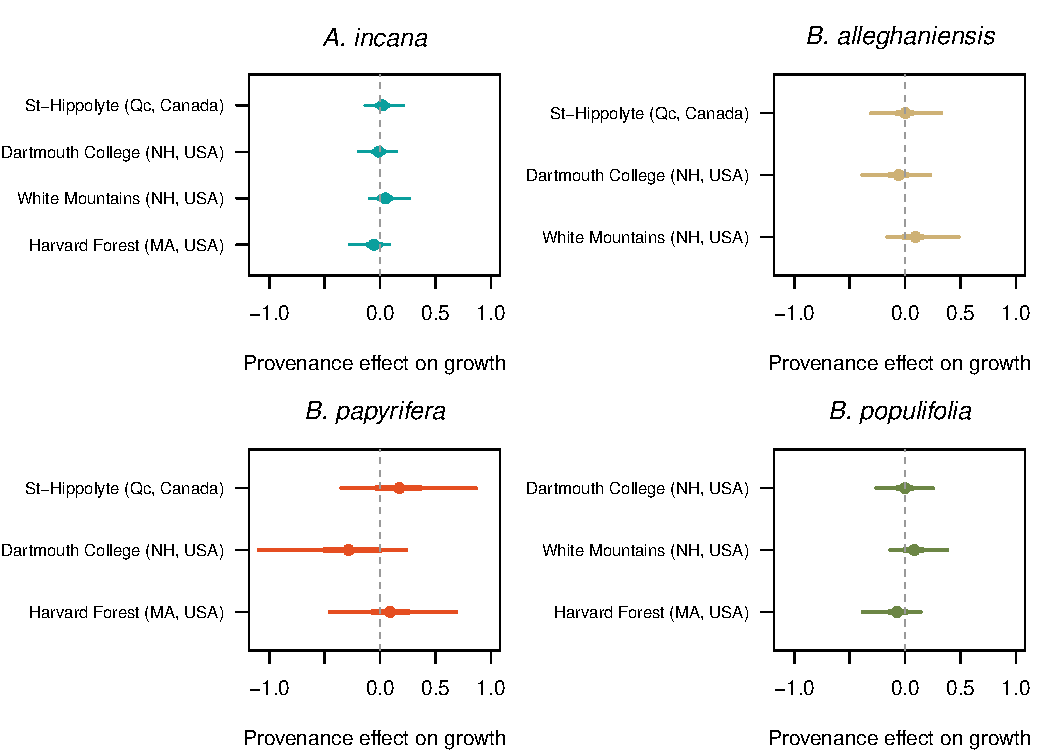
\includegraphics[width=0.8\textwidth]{../../analyses/figures/growthModelsMain/muProvPerSpp.pdf}
\caption{The effect of provenance on growth across a latitudinal gradient estimated per species. We show the ring width (log(mm)) for each provenance estimated from the following intercept-only model: $log(ringwidth) \sim Normal(\alpha_{provenance} + \alpha_{treeid}, \sigma) $, using the package rstanarm version 2.32.1 \citep{gabryRstanarmBayesianApplied2016}. The dots represent the estimated mean of each provenance (ordered by latitude), with 50\% and 90\% uncertainty intervals (thicker and thinner lines, respectively).}
\label{fig:wcmuplotasitePerSpp}
\end{figure}

% Climate data overlap
\begin{figure}[!ht]
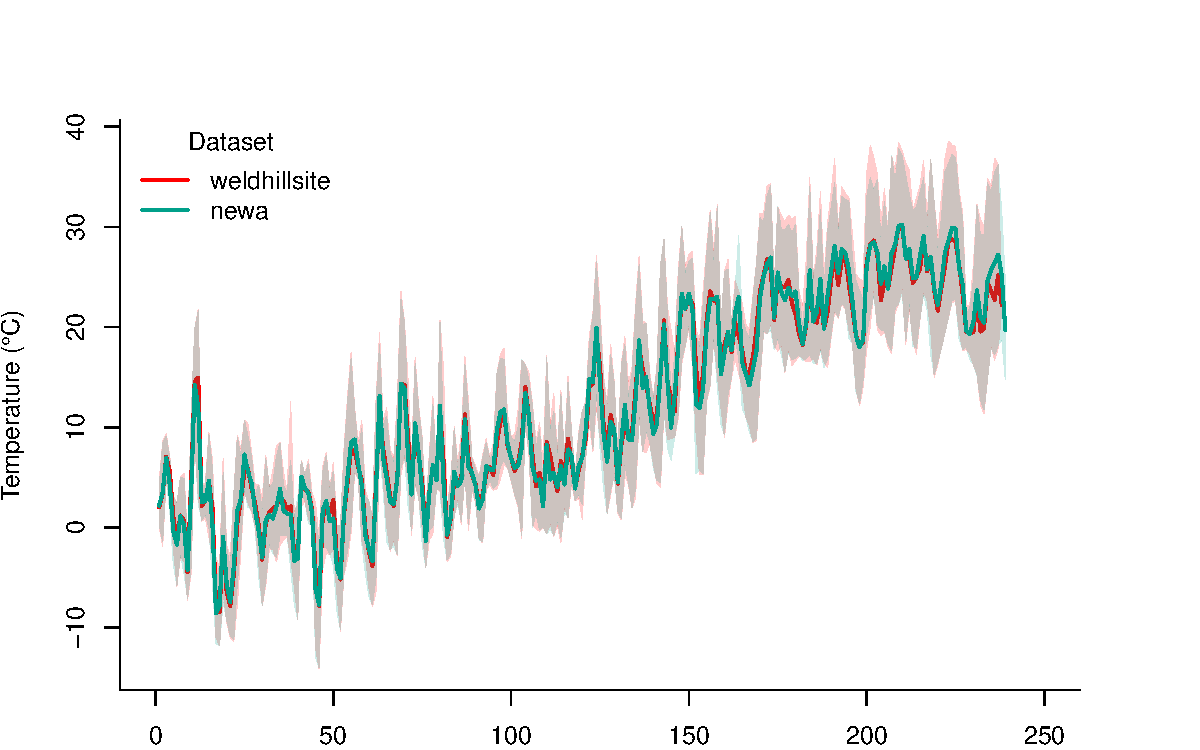
\includegraphics[width=0.9\textwidth]{../../analyses/figures/climate/climateComparison2020.pdf}
\caption{Climate data overlap in 2020 for the two climate stations we used in our dataset (see `Data analyses' section for more details). The lines represent the daily mean temperature of each climate station and the shaded area, the minimum and maximum daily temperatures.}
\label{fig:climOverlap}
\end{figure}

% Z-scored slope results Wildchrokie
\begin{figure}[!ht]
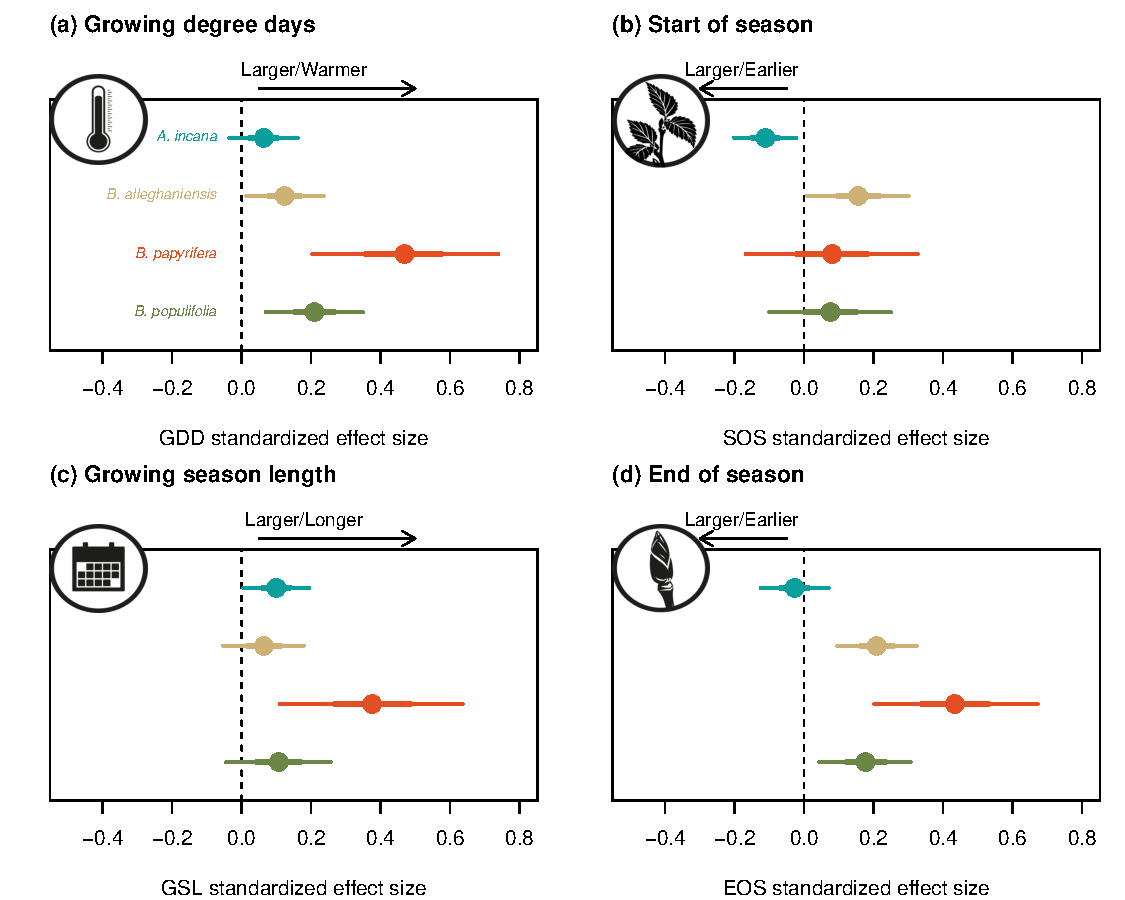
\includegraphics[width=0.8\textwidth]{../../analyses/figures/growthModelsMain/zscored/muALLbsppZ.pdf}
\caption{Effect size of each predictor across our four species. We depict ring width (log(mm)) change per adjusted predictor ($z$-scored; see `Data analyses' section in Methods for more details) for each species. We report mean model slope estimates for each species (dots) with 50\% and 90\% uncertainty intervals (thicker and thinner lines, respectively), for each predictor (growing degree days, growing season length, start of season and end of season).
}
\label{fig:bsppZscored}
\end{figure}

% Full vs restricted data comparison for Wildchrokie
\begin{figure}[!ht]
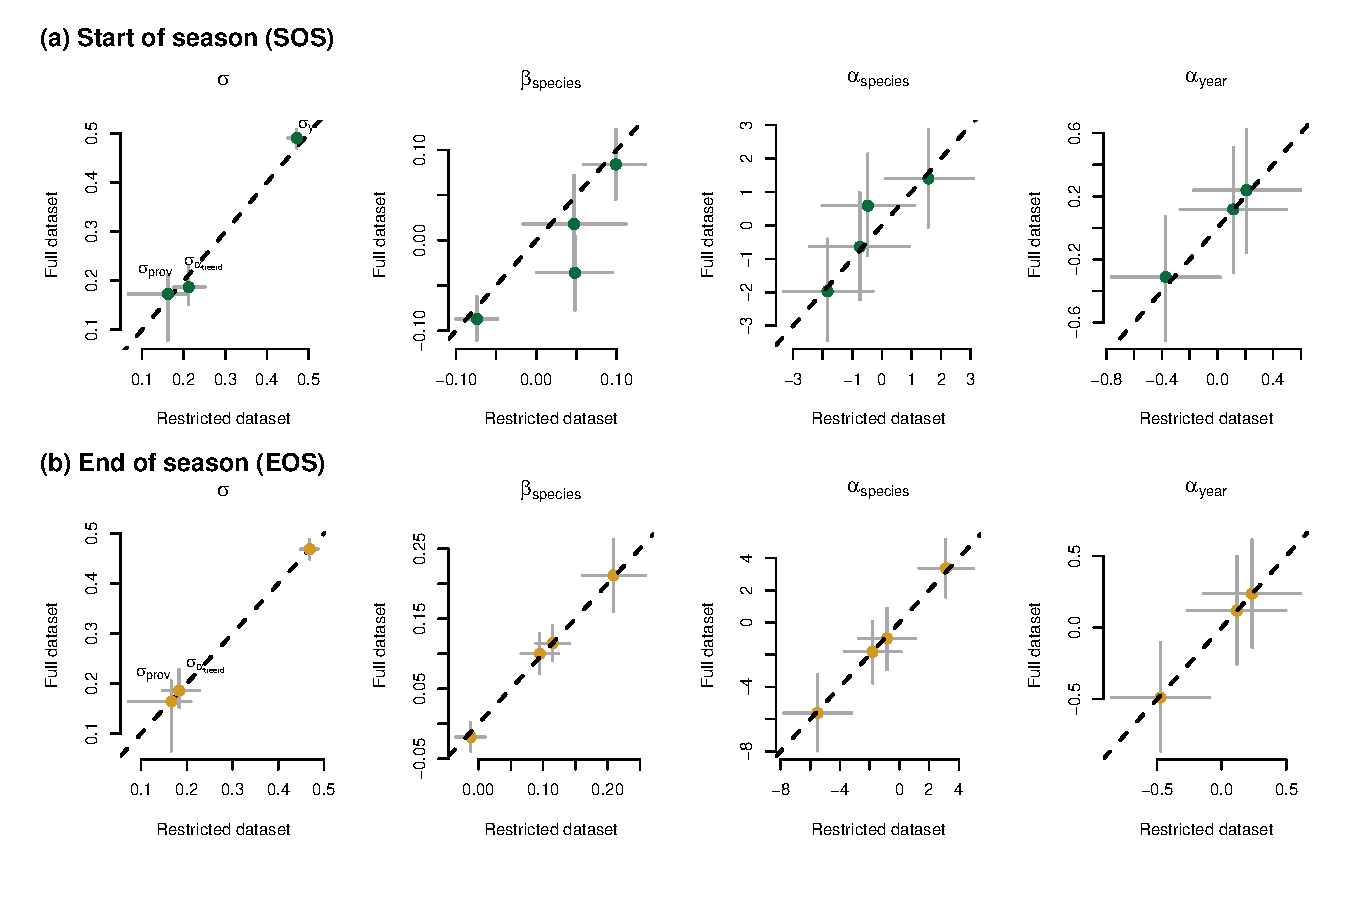
\includegraphics[width=1\textwidth]{../../analyses/figures/growthModelsMain/FullVSRestricted.pdf} 
\caption{Full vs most restricted datasets for the model with start of season (a-d) and end of season (d-h) as the predictor. Each panel represent the different parameters used to fit the models. $\sigma$ (a, e), $\alpha_{species}$ (c, g) and $\alpha_{year}$ (d,h) represent the ring width (log(mm)) for species and year, respectively. $\beta_{species}$ (b, f) represent the change in ring width (log(mm))/adjusted predictor, for each species (see `Data analyses' section in Methods for more details).} 
\label{fig:wcSOSEOScomparison}
\end{figure}

% Figure mu atreeid full
\begin{figure}[!ht]
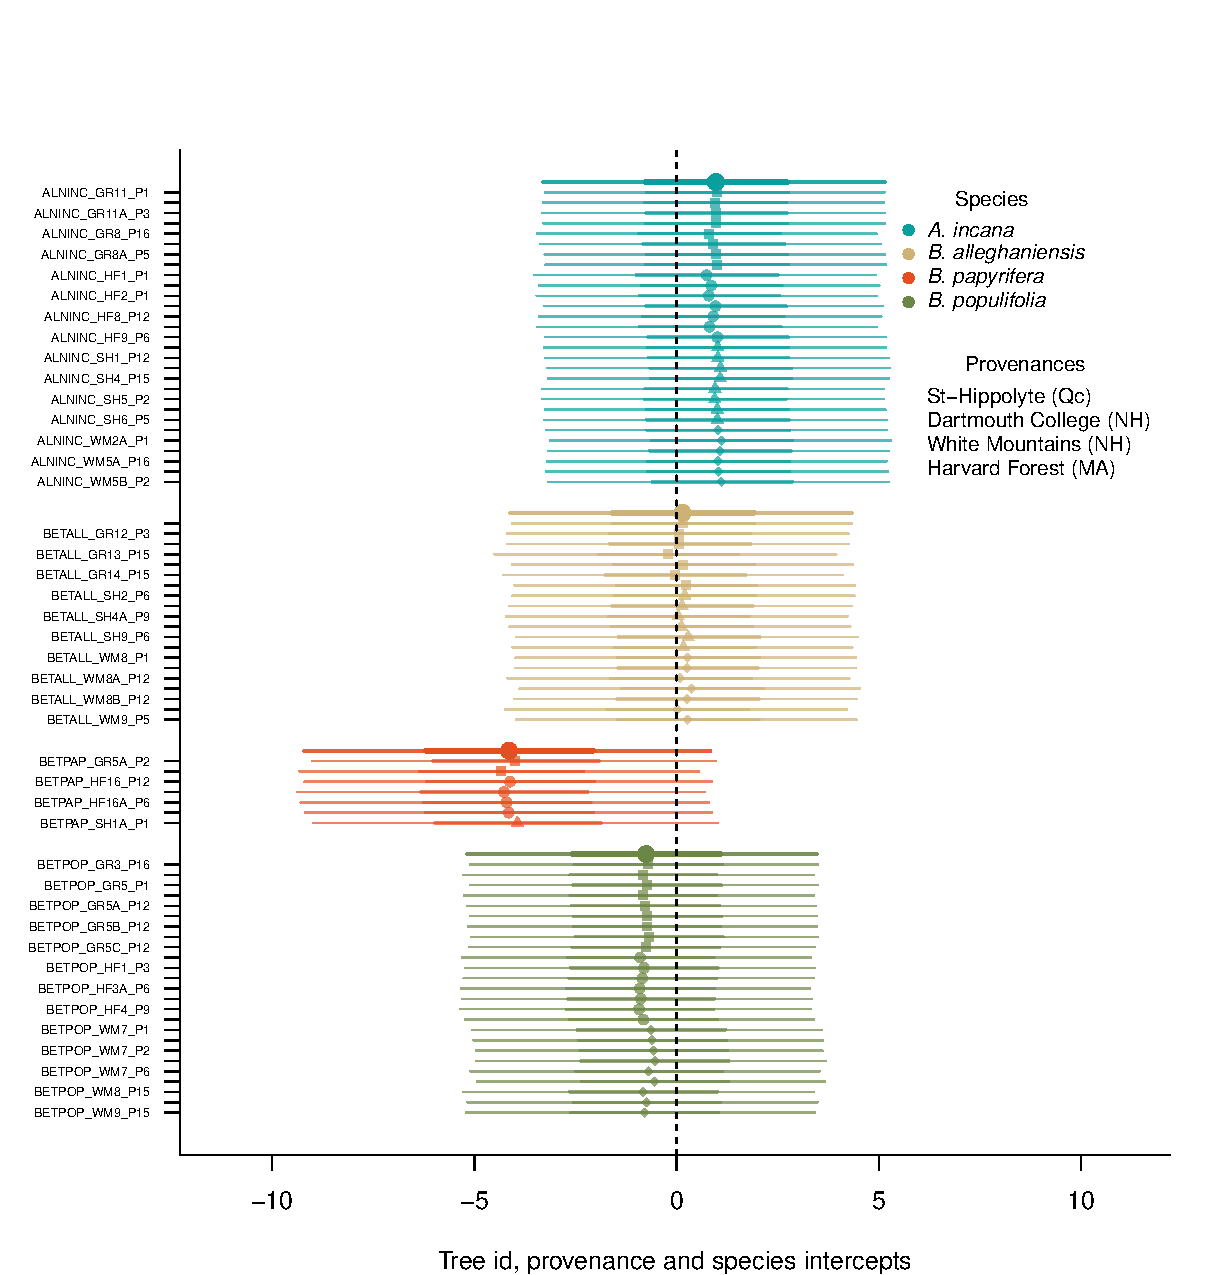
\includegraphics[width=0.8\textwidth]{../../analyses/figures/growthModelsMain/meanPlotGrowthGDD_treeidBYspp.pdf}
\caption{Ring width (log(mm)) deviations from the grand mean for grouping factor of the GDD model. The different tree id values represent the combined intercepts of tree id, provenance, species and averaged year intercepts. The larger dots and lines represent the species intercepts which are the species level estimates averaged across all of their tree ids. The dots are the mean of the posterior distribution and the thick and thin lines, the 50 \% and 90\% uncertainty intervals.}
\label{fig:wcmuplotatreeid}
\end{figure}

% XY facetted by species GDD
\begin{figure}[!ht]
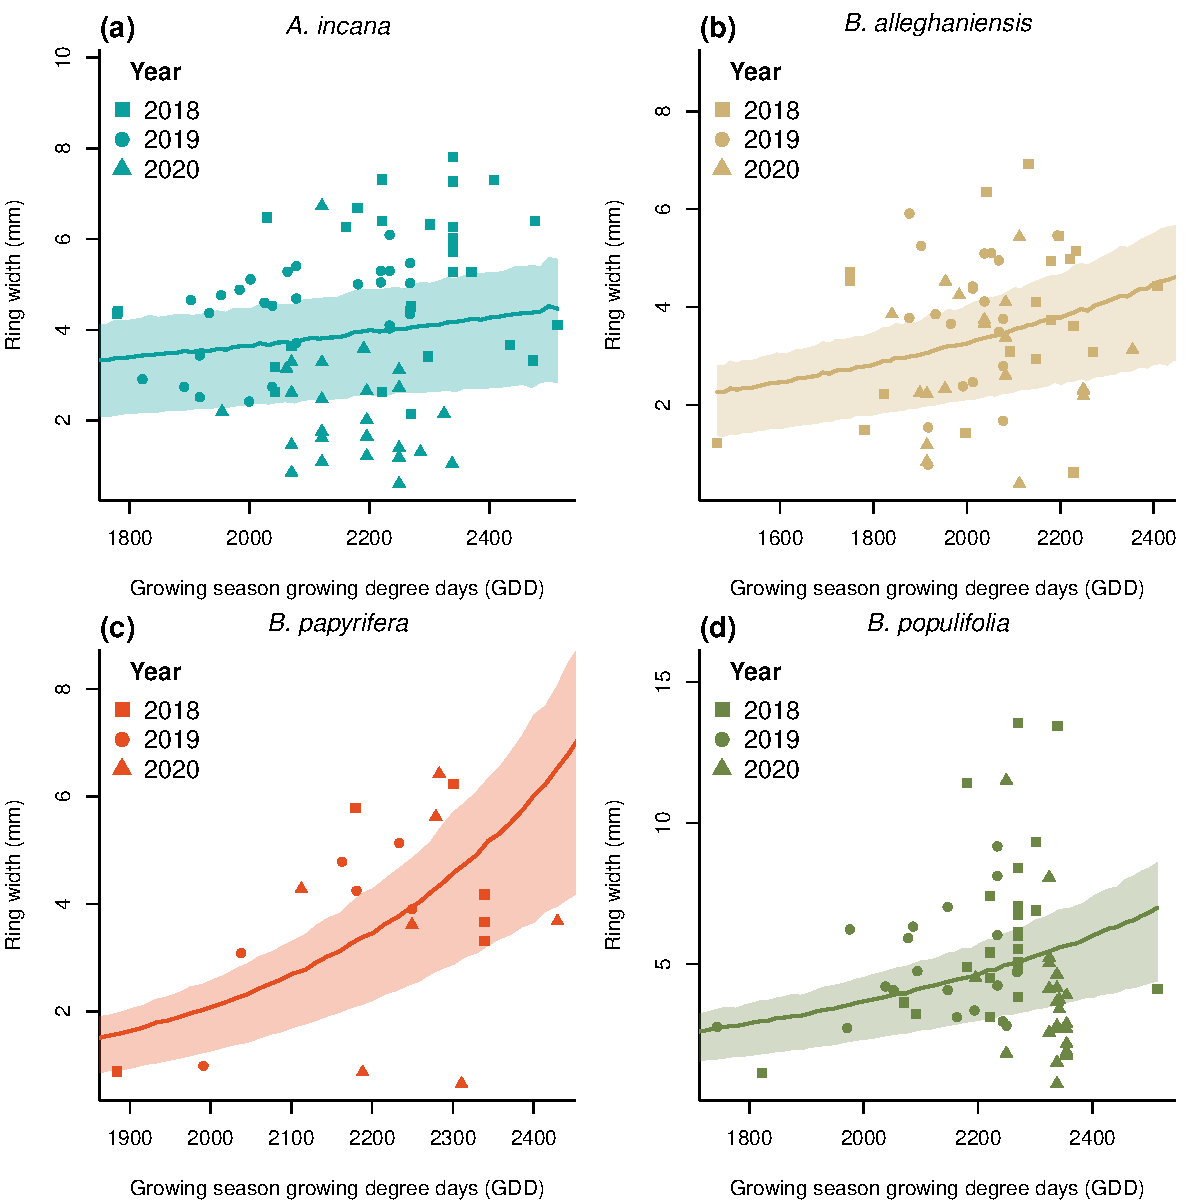
\includegraphics[width=0.8\textwidth]{../../analyses/figures/growthModelsMain/growthModelSlopesperSppFacet.pdf}
\caption{Ring width (mm) trends in response to thermal season (growing degree days). The lines represent the mean of the posterior distribution and the shaded area, the 50\% uncertainty intervals at each predictor value back-converted from the model which uses ring width in log(mm) as the response variable. The dots are the empirical data shaped by year.}
\label{fig:wcxyGDD}
\end{figure}

% XY facetted by species GSL
\begin{figure}[!ht]
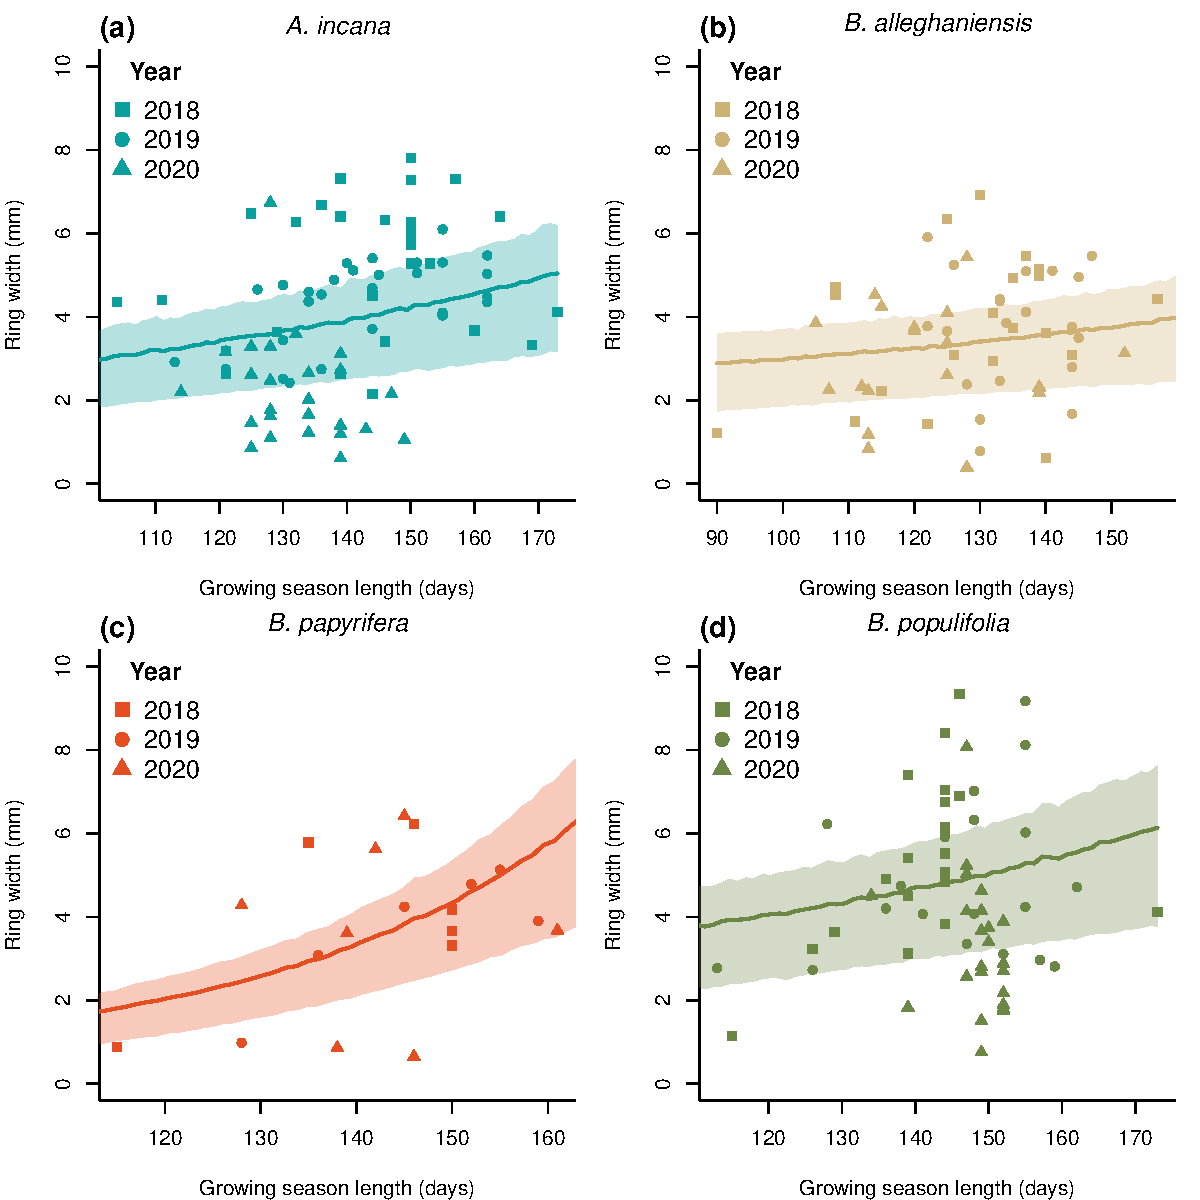
\includegraphics[width=0.8\textwidth]{../../analyses/figures/growthModelsMain/growthModelSlopesperSppFacetGSL.pdf}
\caption{Ring width trends (mm) in response to calendar season (growing season length). The lines represent the mean of the posterior distribution and the shaded area, the 50\% uncertainty intervals at each predictor value back-converted from the model which uses ring width in log(mm) as the response variable. The dots are the empirical data shaped by year.}
\label{fig:wcxyGSL}
\end{figure}

%<><><><><><><><><><><><><><><><><><><><><><><><><><><><><><><><><><><><><><><><>
% REFERENCES %
%<><><><><><><><><><><><><><><><><><><><><><><><><><><><><><><><><><><><><><><><>
\clearpage 

\bibliography{ExportedItems}
\bibliographystyle{besjournals} 


\end{document}
